% This must be in the first 5 lines to tell arXiv to use pdfLaTeX, which is strongly recommended.
\pdfoutput=1
% In particular, the hyperref package requires pdfLaTeX in order to break URLs across lines.

\documentclass[11pt]{article}

% JackDann: Use Chinese Character support package
\usepackage{CJKutf8}

% JackDann: Use Algorithmic support package
\usepackage{algpseudocode}
\usepackage{algorithm}
% Remove the "review" option to generate the final version.
\usepackage[review]{ACL2023}

% Standard package includes
\usepackage{times}
\usepackage{latexsym}

% For proper rendering and hyphenation of words containing Latin characters (including in bib files)
\usepackage[T1]{fontenc}
% For Vietnamese characters
% \usepackage[T5]{fontenc}
% See https://www.latex-project.org/help/documentation/encguide.pdf for other character sets

% This assumes your files are encoded as UTF8
\usepackage[utf8]{inputenc}

% This is not strictly necessary, and may be commented out.
% However, it will improve the layout of the manuscript,
% and will typically save some space.
\usepackage{microtype}

% This is also not strictly necessary, and may be commented out.
% However, it will improve the aesthetics of text in
% the typewriter font.
\usepackage{inconsolata}

% Jack Dann
% To use Dui and Cuo, use this package XD
\usepackage{bbding}

% Jack Dann
% To use picture and tables use these package
\usepackage{graphicx}
\usepackage{multirow}
\usepackage{multicol}
\usepackage{booktabs}
\usepackage{amsmath}

% If the title and author information does not fit in the area allocated, uncomment the following
%
%\setlength\titlebox{<dim>}
%
% and set <dim> to something 5cm or larger.

\title{From Text to CQL: Bridging Natural Language and \\Corpus  Search Engine}

% Author information can be set in various styles:
% For several authors from the same institution:
% \author{Author 1 \and ... \and Author n \\
%         Address line \\ ... \\ Address line}
% if the names do not fit well on one line use
%         Author 1 \\ {\bf Author 2} \\ ... \\ {\bf Author n} \\
% For authors from different institutions:
% \author{Author 1 \\ Address line \\  ... \\ Address line
%         \And  ... \And
%         Author n \\ Address line \\ ... \\ Address line}
% To start a seperate ``row'' of authors use \AND, as in
% \author{Author 1 \\ Address line \\  ... \\ Address line
%         \AND
%         Author 2 \\ Address line \\ ... \\ Address line \And
%         Author 3 \\ Address line \\ ... \\ Address line}

\author{First Author \\
  Affiliation / Address line 1 \\
  Affiliation / Address line 2 \\
  Affiliation / Address line 3 \\
  \texttt{email@domain} \\\And
  Second Author \\
  Affiliation / Address line 1 \\
  Affiliation / Address line 2 \\
  Affiliation / Address line 3 \\
  \texttt{email@domain} \\}

\begin{document}
\begin{CJK*}{UTF8}{gbsn}
\maketitle
\begin{abstract}
Natural Language Processing (NLP) technologies have revolutionized the way we interact with information systems, with a significant focus on converting natural language queries into formal query languages such as SQL. However, less emphasis has been placed on the Corpus Query Language (CQL), a critical tool for linguistic research and detailed analysis within text corpora. The manual construction of CQL queries is a complex, time-intensive task requiring deep expertise, presenting a notable challenge for both researchers and practitioners. This paper presents the first text to Corpus Query Language (CQL) task, aiming to automate the translation of natural language into CQL. We present a comprehensive framework for this task, including a specifically curated large-scale dataset and methodologies leveraging large language models (LLMs) for effective text-to-CQL conversion. Moreover, we establish advanced evaluation metrics to assess the syntactic and semantic accuracy of the generated queries. Our contributions include not only a rich dataset facilitating benchmarking but also innovative LLM-based conversion approaches and thorough experiments. The results demonstrate the efficacy of our methods and provide insights into the complexities of text-to-CQL conversion.
\end{abstract}





\section{Introduction}

Natural Language Processing~(NLP) technologies have significantly enhanced our interaction with information systems, enabling a more intuitive and effective interface for communicating with computers. Among these advancements, the conversion of natural language queries into query languages, such as Structured Query Language~(SQL) for databases, has been a focal point of research. The exploration of linguistic corpora has significantly benefitted from advancements in query languages, enabling researchers and practitioners to navigate and analyze text corpora efficiently. While several query languages, such as SQL for databases and various Domain-Specific Languages (DSLs) for other applications, have seen extensive study and application, the focus on Corpus Query Language (CQL) has been relatively less pronounced. Existing research has richly explored Text-to-SQL\citep{zhong2017seq2sql, liu2022tapex, yu-etal-2018-spider, li2023resdsql, gao2023texttosql, pourreza2023dinsql, dong2023c3, li2023can} and Text-to-DSL\citep{wang2023grammar, staniek2023texttooverpassql} tasks, demonstrating the feasibility and efficiency of translating natural language instructions into formal query statements to interact with databases and information systems.

\begin{figure}[t]
    \centering
    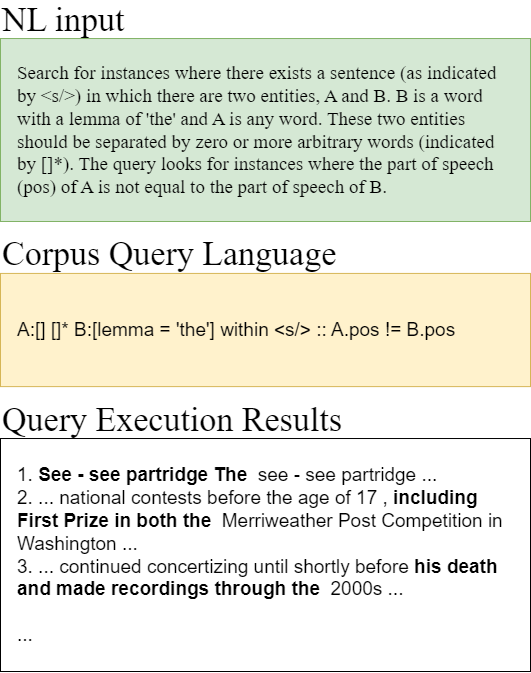
\includegraphics[width=3in]{CQL.drawio.pdf}
    \caption{Example task diagram. Given any input natural language query description, the model is expected to convert it into the corresponding Corpus Query Language (CQL) and the generated CQL should be able to be accurately executed by the Corpus Engine. The CQL uses symbols (in green) with a small number of CQL uses symbols (green) and a small number of keywords (purple) to construct queries, and allows to specify names (blue) for tokens to constrain relationships between tokens. Execution Results are the results returned by Blacklab when executing the CQL on the En-Wiki corpus.}
    \label{fig:cql}
\end{figure}


CQL is vital for linguistic research as it offers a nuanced approach to querying annotated text corpora, allowing for sophisticated searches based on linguistic features. This capability is crucial for conducting detailed linguistic analysis and supports a wide range of research activities in NLP and computational linguistics. However, crafting CQL queries manually is a time-consuming and error-prone process, necessitating a high level of expertise in both the query language and the specific annotations of the corpus being queried.

Recognizing the challenges associated with manual query construction and the potential for automation, this work introduces the task of Text-to-CQL conversion. This task aims to bridge the gap between natural language descriptions and their corresponding CQL representations, facilitating more accessible and efficient interactions with linguistic corpora with rich linguistic annotations. However, unlike its counterparts in Text-to-SQL conversion, the Text-to-CQL task faces unique challenges, including a scarcity of dedicated training data and the intricate syntax and semantics of CQL, which are not readily handled by even the most advanced generative models, such as GPT-4, without specialized training and adaptation.
The models need not only to understand the semantics of natural language descriptions but also to navigate the complexities of linguistic annotations and the specific query constructs of CQL.

This work aims to address these challenges by proposing a comprehensive framework for Text-to-CQL conversion. We introduce a novel dataset specifically curated for this task, alongside methodologies and evaluation metrics tailored to the unique requirements of CQL query generation. Our contributions include the creation of a large-scale dataset that encompasses a wide range of linguistic phenomena and query types, the development of models that adapt large language models and introduce new LLM-based approaches for Text-to-CQL conversion, and the establishment of evaluation metrics that go beyond traditional measures to assess the syntactic validity and semantic correctness of the generated queries.

In summary, our key contributions are as follows:
\begin{itemize}
    \item A large-scale, diverse dataset for Text-to-CQL conversion, providing a benchmark for model evaluation.
    \item A series of LLM-based Text-to-CQL methodologies, including both prompt engineering and fine-tuning pre-trained language models.
    \item New evaluation metrics designed to accurately reflect the complexities of Text-to-CQL conversion, focusing on syntactic validity and semantic correctness.
    \item Comprehensive experiments and analysis that highlight the effectiveness of our proposed methods and offer insights into the challenges of Text-to-CQL conversion.
\end{itemize}

Through these contributions, we seek not only to advance the state of the art in automatic query generation for linguistic corpora but also to facilitate broader access to these valuable resources for researchers across NLP and computational linguistics. We hope that our work could enable novel applications and foster interdisciplinary research collaborations by simplifying the access to and manipulation of linguistic corpora.

We have released all our code and datasets for research purposes at ...


\section{Related Work}
\label{sec:related_work}

\subsection{Text-to-SQL}
\label{sec:text2sql}

Text-to-SQL conversion, a key research area, involves translating natural language questions into SQL queries. 
Seq2SQL~\citep{zhong2017seq2sql} is a notable model in this field, utilizing policy-based reinforcement learning to accurately generate SQL queries, particularly focusing on the unordered nature of query conditions. 
It excelled in both execution and logical form accuracy on the WikiSQL dataset.
In the same data set, TAPEX~\citep{liu2022tapex}, an execution-centric table pretraining approach that learns a neural SQL executor over a synthetic corpus, achieved the state-of-the-art results.

The Spider~\citep{yu-etal-2018-spider} dataset furthered Text-to-SQL research by presenting a complex, cross-domain semantic parsing challenge. 
It features varied SQL queries and databases, pushing models to adapt to new structures and databases. 
RESDSQL~\citep{li2023resdsql} introduced a ranking-enhanced encoding and skeleton-aware decoding framework that effectively decouples schema linking and skeleton parsing, demonstrating improved parsing performance and robustness on the Spider dataset and its variants.

Recent advances in large language models (LLMs), such as GPT-4~\citep{openai2023gpt4} and Claude-2, have also shown impressive results in this domain~\citep{gao2023texttosql, pourreza2023dinsql, dong2023c3}. 
To our knowledge, most previous benchmarks, including Spider and WikiSQL, focused on database schemas with limited rows, creating a gap between academic studies and real-world applications. 
To bridge this gap, the BIRD~\citep{li2023can} benchmark was introduced, providing a comprehensive text-to-SQL dataset that emphasizes the challenges of dealing with dirty and noisy database values, grounding external knowledge, and ensuring SQL efficiency in massive databases.

However, adapting these methods from Text-to-SQL to Text-to-CQL isn't straightforward, primarily because of the scarcity of training data for Text-to-CQL. 
This challenge motivated the proposal of this paper.

\subsection{Text-to-DSL}
\label{sec:text2dsl}

The field of generating Domain-Specific Languages (DSLs) from natural language, known as Text-to-DSL, has seen a surge in interest, primarily due to the emergence of LLMs capable of understanding and generating structured languages. 
A notable approach in this area is Grammar Prompting~\citep{wang2023grammar}, which leverages Backus–Naur Form (BNF) grammars to provide LLMs with domain-specific constraints and external knowledge. 
This method has shown promise across various DSL generation tasks, including semantic parsing and molecule generation.

Text-to-OverpassQL~\citep{staniek2023texttooverpassql} focused on generating Overpass queries from natural language. 
This task is particularly challenging due to the complex and open-vocabulary nature of the Overpass Query Language (OverpassQL), which is used to query the OpenStreetMap (OSM) database. 
\citet{staniek2023texttooverpassql} proposed the OverpassNL dataset, consisting of 8,352 queries with corresponding natural language inputs, and established task-specific evaluation metrics to assess the performance of sequence generation models in this context.

Transitioning methodologies from Text-to-DSL to Text-to-CQL is notably challenging, largely because of the limited training data for Text-to-CQL and the intrinsic complexity of CQL. 
This complexity demands the creation of specialized datasets, models, and algorithms tailored for Text-to-CQL.


\section{Background}


 Corpus Query Language (CQL) is a query language specifically used to query corpus with linguistic features required by users. The CQL utilized in this article primarily pertains to the BlackLab Corpus Query Language. The existing systems for Corpus Query Languages are offshoots of the Corpus Query Language Processor (CQP) query language, which is a suite of languages designed for the retrieval of lexical information. Numerous corpus search tools endorse and employ CQL, including well-known platforms such as CQPweb, Sketch Engine, and BlackLab, among others. Some examples of CQL are shown in Table \ref{tab:CQLexample}.



\begin{table*}
    \centering
    \begin{tabular}{p{5em}p{15em}p{15em}} 
    \hline
    \textbf{Type} & \textbf{CQL} &\textbf{NL} \\
    \hline
    Simple & \verb|[lemma="teapot"]| &Find the lemma teapot.\\
    Within & \verb|[pos="N.*"]|\verb|within|\verb|[pos="VB.*"]| \verb|[]|\verb|{0,5}|\verb|[pos="VB.*"]| & Searches for nouns that appear between two verbs to be, the verbs are at a distance of max. 5 tokens from each other.\\
    Condition & \verb|1:[] 2:[] :: 1.tag = 2.tag| & Find any two tokens whose tag is the same.\\
    \hline
    \end{tabular}
    \caption{Example of the Corpus Query Language. The above examples and explanations are all from the Sketch Engine documentation. }
    \label{tab:CQLexample}
\end{table*}

 

\subsection{CQL Statementes}
\citet{pourreza2023dinsql} categorized SQL into Simple, Complex, and Nested classes, delineating distinctions in sentence structure complexity within the Text-to-SQL task. Analogously, CQL can be classified into three categories based on keywords, as distinct keywords induce alterations in the CQL structure.

\textbf{Simpe Query.} In CQL, users possess the capability to formulate queries targeting the desired corpus by leveraging the sequential associations among tokens. Each token is represented by a pair of square brackets, and the filtering conditions of the token are represented by key-value expressions and logical operators in square brackets. For example, to retrieve instances of research categorized as nouns within the corpus, the ensuing CQL expression may be employed (pos tag takes CTB part-of-speech system as an example):

\verb|[word='research' & pos='NN']|

In the above example, we employed a corpus aligned with the Penn Treebank (PTB) \citep{ptb} lexical labeling system. It is worth noting that various corpora may employ different annotation systems. The model's capacity to accurately associate the lexical properties of natural language representations with the appropriate lexical labels represents a potential challenge.

\textbf{Within Query.} As shown in Table \ref{tab:CQLexample}, the "within" syntax serves to partition a CQL statement into two sub-queries, restricting the target retrieved in the initial portion to the scope delineated in the subsequent segment. Typically, "within" is accompanied by a sub-query with a larger maximum target length or certain XML structure. Notably, within structures allow nesting.

\textbf{Condition Query.} A condition statement is employed to compare tokens with each other and to impart additional options to individual tokens. All attributes of a token are eligible for comparison within a condition, and conditions within a query can be linked using logical operators.

\subsection{Task Formulation}

Given a parallel dataset of natural language descriptions and CQL queries $D = \left\{(X_i, Y_i)\right\}_{i=1}^N$, where $X_i = \left\{w_1, w_2, \ldots, w_{n_1}\right\}$ is a query described in natural language, and $Y_i = \left\{t_1, t_2, \ldots, t_{n_2}\right\}$ is the CQL corresponding to the NL. $n_1$ represents the length of the natural language description while $n_2$ represents the length of the CQL query. The goal of the Text-to-CQL task is to train a generative model that converts a natural language query description into a query language. This also means that the model needs to have the ability to extract key information from a natural language description and combine it into CQL with the correct syntax, as well as convert an unseen sentence into a correct CQL query.


% JackDann@2024-1-16
% Section Dataset
\section{Data Acquisition }
\subsection{Corpus Collection}
We employed two distinct corpora for our study, one in the Chinese and the other in English. Both corpora were annotated using Stanford Corenlp.

\textbf{TCFL Textbook.} We collected the mainstream teaching materials for teaching Chinese as a foreign language on the market and constructed the TCFL corpus.


\begin{table}[h!]
\centering
\begin{tabular}{lcc}
\toprule
\textbf{Dataset} & \textbf{Sentence Count} & \textbf{Token Count}\\
\midrule
TCFL Textbook & 578,358 & 7,731,686  \\
EnWiki & 138,616,990 & 3,142,382,778  \\
\bottomrule
\end{tabular}
\caption{Dataset Statistics.}
\label{tab:corpusScale}
\end{table}



\textbf{EnWiki.} We use the EnWiki\citep{enwiki}\footnote{ https://dumps.wikimedia.org/} corpus and clean and extract the text in it using wiki-extractor\footnote{https://github.com/attardi/wikiextractor}\citep{Wikiextractor2015}. The EnWiki contains 1.9 billion words in more than 4.4 million articles.

Our Text-to-CQL dataset is divided into two parts: Chinese NL-CQL pairs based on TCFL corpus and English NL-CQL pairs based on EnWiki corpus.
\subsection{CQL Generation Strategies}

Certain conventional dataset construction methods, such as the data mining techniques employed in WikiTable\citep{wikitable}, are precluded due to the limited availability of pertinent information on the Internet. Simultaneously, other approaches reliant on syntax-based automated data generation, frequently employed in program testing, are rendered impracticable owing to inherent deficiencies in the logic of the resultant data. Consequently, we put forth a novel data collection approach grounded in Chinese collocation extraction.

\subsubsection{Collocation Extraction}

Our approach to data augmentation is based on Chinese Collocation Extraction\citep{hucollocation}. An example of Chinese collocation extraction is shown in table \ref{tab:collexample}. The collocation set encompasses four distinct properties and nine types of Chinese collocations, and extraction methodology leveraging both surface and dependency relation knowledge, along with statistical methods. Furthermore, we incorporate Chinese enhanced dependency\citep{yujingsi} to enhance the efficacy of collocation extraction. Specifically, our process involves initially employing Stanford CoreNLP\citep{corenlp} for the dependency analysis of sentences within the corpus. Subsequently, enhanced dependencies are introduced, and collocations are extracted from the entire corpus. Finally, a random selection is made from the extracted collocations and applied in classified CQL templates.

\begin{table}
    \centering
    \begin{tabular}{lp{9em}p{9em}} 
    \hline
    \textbf{Collocation Text} & \textbf{Collocation Type} \\
    \hline
    所以说\_AD	X	有\_VE	&D\_X\_V \\
    各\_AD	有\_VE	& D\_V \\
    有\_VE	利弊\_NN	& V\_O \\ 
    \hline
    \end{tabular}
    \caption{A simple example of collocation extraction of the input sentence '
    所以说各有利弊吧。'. Input a natural language sentence and the collocation extraction program gives a set of word combinations from the sentence. There is a dependency-based relationship between these word combinations. The X in the first collocation means there are other words between the two collocation words.}
    \label{tab:collexample}
\end{table}

\subsubsection{CQL Template}
As depicted in Table \ref{tab:CQLexample}, the CQL queries can be categorized into three distinct types: simple, within, and condition. In alignment with these three CQL types, we established distinct templates tailored to each type.

\textbf{Simple Statements. }
Given that the collocations extracted from the corpus consist of word combinations exceeding two words, our post-extraction procedure involves traversing the word sequence.
Initially, we implement a filtering process for the extracted collocations. A certain collocation is excluded if the frequency of any constituent word within the collocation has a low frequency within the corpus. Subsequently, we introduce tokens without any criteria randomly between collocated words and randomly determine the number of repetitions. Finally, we randomly assign a set of conditions for each token. For any token (such as noun 'book'), we randomly convert it into the following forms:
\begin{enumerate}
\item Simple word query (W).
\item Simple part-of-speech query (P).
\item Query its word and POS at the same time. The logical relationship between the two conditions is randomly chosen from \emph{AND} (WAP) or \emph{OR} (WOP).
\item Query two words at the same time, and there is an OR relationship between them (WW). In this case, we also randomly restrict its part of speech with an AND relation (WWP). Another candidate word is selected based on the synonyms specified in the synonym forest.

\end{enumerate}

Examples was shown in Table \ref{tab:simpleTokenExample}. After converting the word in each collocation to CQL, we randomly add empty tokens to it as shown in Algorithm \ref{alg:cap}, where the $mutate$ function refers to the process of converting the collocation word to a CQL token as described in this section and the $insert\_null\_token$ method randomly adds an unrestricted token to the end of a CQL and assigns it a random number of repetitions or quantifiers using regular expressions.

\begin{table}
    \centering
    \begin{tabular}{p{3em}p{15em}} 
    \hline
    \textbf{Token Query Type} & \textbf{CQL} \\
    \hline
    W& \verb|[word='book']| \\
    P& \verb|[pos='NN']|\\
    WOP& \verb^[word='book'|pos='NN']^\\
    WAP& \verb^[word='book'&pos='NN']^\\
    WW& \verb^[word='book'|word=^ \verb^'notebook']^\\
    WWP& \verb^[(word='book'|word=^ \verb^'notebook')&pos='NN']^\\

    \hline
    \end{tabular}
    \caption{An example of a CQL Token Queries transformed from Token extracted from a corpus, containing 6 random transformations: simple Word Query (W), Simple Pos Query (P), Word and Pos Query (WAP),Word or Pos Query (WOP), Word or Word query (WW) and Words with Pos Query (WWP)}
    \label{tab:simpleTokenExample}
\end{table}

\begin{algorithm}
\caption{Generation of simple CQL}\label{alg:cap}
\begin{algorithmic}
\Require $Collocation = \left\{ w_1, w_2, \ldots, w_n \right\}$
% \Ensure $y = x^n$
% \State $y \gets 1$
% \State $X \gets x$
% \State $N \gets n$
\State $CQL\gets None $ 
\While{$i \neq 0$}
\If{$freq(w_i) \leq 5 $}
    \State $Abandon()$
\Else
    \State $CQL.append(Mutate(w_i))$
    \If{$w_{i+1} = "X"$}
        \State CQL.insert\_null\_token()
        \State $i \gets i + 1$    
    \Else
        \If $random\_number \lt 0.5$
            \State CQL.insert\_null\_token()
        \EndIf
        \EndIf
    \State $i \gets i + 1$
\EndIf
\EndWhile
\end{algorithmic}
\end{algorithm}

\textbf{Within Statements. }
Two potential subqueries are permissible following the keyword \verb|within|:
 1) \textbf{Simple CQL Subquery.} This causes the corpus searching engine to search for CQL before the \verb|within| keyword within the specified Subquery scope. 
 2) \textbf{Structure.} One may utilize XML Structure to confine the query scope to the specified XML domain, with strict prohibition on extending beyond the boundaries defined by the tags. Concurrently, the incorporation of conditions for filtering XML attribute values within the XML Structure is also permissible. 

For both cases, we randomly apply one of them. On one hand, two CQLs are generated through collocation analysis, wherein the maximum token length they can reference is examined. Then the shorter one is positioned preceding the \verb|within| keyword, while the longer one is positioned thereafter. On the other hand, we randomly specify a certain level of XML format and place it after the keyword. 

We also generate nested "within" statements. however, nesting multiple levels of queries may lack meaningful interpretation and pose challenges in natural language description. Furthermore, XML structures are commonly segmented at the sentence level and beyond, rendering queries across XML structures practically insignificant. Consequently, we restrict the generation of nested queries to those comprising two "within" keywords, with the XML structure query positioned at the end of the query (representing the highest priority decision). An example of our generated \emph{within} CQL is shown in Table \ref{tab:within_example}

\begin{table}
    \centering
    \begin{tabular}{|p{3em}|p{15em}|} % 第一列最大宽度为四个字母
    \hline
    \textbf{CQL} &[word = 'evening'] [pos = 'NN']  within  [word != 'real' \& pos = 'RB'] []{4,7} [word != 'downside' \& pos = 'NN'] within  <s/>   \\
    \hline
    \textbf{NL}&  Find sentences where the word 'evening' followed by a noun,which occurred within a range of 4 to 7 words post adverb that is not word 'real' ,before a noun that is not word 'downside'. \\
    \hline
    \end{tabular}
    \caption{Examples of generated \emph{within} CQL.A CQL with the condition keyword may have a long query length.}
    \label{tab:within_example}
\end{table}


\textbf{Condition Statements. }
we extract the analytical outcomes of all sentences within the corpus. From these results, we identify token pairs within sentences where parts of speech or words share equality. Subsequently, sentences containing such token pairs are randomly selected, and CQL with Condition syntax is generated based on these equivalence relationships. Given that the collocation-based method is no longer applicable to CQL with equivalence relationships, our consideration is confined to scenarios involving the embedding of CQL within the XML structure in condition statements.An instance of our generated condition CQL is shown in Table~\ref{tab:condition_example}.

\begin{table}
    \centering
    \begin{tabular}{|p{3em}|p{15em}|} % 第一列最大宽度为四个字母
    \hline
    CQL & A:[] []? B:[] within <s/> :: A.pos = B.pos \\
    \hline
    NL & Find corpus in which there are zero or one arbitrary words between two words of the same part of speech in a sentence. \\
    \hline
    \end{tabular}
    \caption{Examples of generated \emph{condition} CQL.}
    \label{tab:condition_example}
\end{table}

\subsection{Annotation}

To ensure clarity and precision in the natural language descriptions, we implemented a training and selection process for our annotators. Out of the initial pool of 14 recruited annotators, we assessed their abilities and ultimately retained eight annotators for the subsequent annotation tasks. These annotators all have undergraduate degrees and are familiar with both computer science and linguistics.

In an effort to ensure the diversity and authenticity of our queries, we did not place any language style restrictions on the annotators. This approach aimed to capture a wide range of natural language expressions that mirror how individuals interact with corpus in practice.

Simultaneously, with the paramount objective of maintaining annotation precision, each CQL underwent annotation by two separate annotators and was subjected to review by two annotators proficient in CQL. The most accurate and refined annotations were then retained in our dataset.

\section{Experiments}
In the construction of the Text-to-CQL dataset, we implemented five distinct methodologies, encompassing approaches based on the In Context Learning (ICL) Method and approaches using pretraining or fine-tuning pre-trained language models.

\subsection{In-Context Learning (ICL) Methods}

We  investigate three classifications of Large Language Model (LLM) prompt methods to assess the efficacy of LLMs in Text-to-CQL tasks.

\textbf{Direct Inquiry(DI).} 
Requesting the LLM to generate CQL statements from a provided natural language description. In this scenario, no additional information is appended to the prompt.  

\textbf{Documentation Prompt (DP).} Furnish the LLM with a CQL tutorial created by human experts, derived from tutorials accessible in Sketch Engine\citep{sketchengine1,sketchengine2} and Blacklab\citep{blacklab} Documentation. Within the tutorial, elucidate the syntax of CQL using natural language and furnish illustrative instances, sourced from the tutorial documentation.

\textbf{Few-shot ICL.} We adhere to the methodology outlined by \citet{sun2023battle} and three sets of experiments with different numbers of examples were set up. In each group of examples, we set one example for each of the three types of CQL: simple, within, and condition. 1-Shot Learning (1SL) and 3-Shot Learning (SL) means that we embed one or three groups of examples in the prompt. Prompt details can be found in the Appendix \ref{appendix:prompts}.

\subsection{Fine-tuning PLM Methods. }  

The Text-to-CQL task can be conceptualized as a sequence-to-sequence problem, wherein a segment of natural language is mapped onto a CQL query. Models equipped with an encoder-decoder architecture are aptly suited the Text-to-CQL Task. Within this architecture, the encoder functions to interpret the input natural language, whereas the decoder is tasked with autoregressively generating the corresponding CQL query. This category encompasses several models, including BERT\citep{devlin2018bert}, which is characterized by its exclusive use of an encoder; T5\citep{t5} and BART\citep{bart}, which incorporate both an encoder and a decoder; and GPT\citep{radford2019gpt}, distinguished by its sole reliance on a decoder, among others. In selecting an appropriate pre-trained model for the Text-to-CQL conversion task, this study prioritizes BART due to its integrated encoder-decoder architecture. Furthermore, BART's foundation on a denoising autoencoder pre-training paradigm potentially enhances its proficiency in natural language comprehension and structured query generation, as evidenced by preliminary experimental findings.

For the generation of CQL queries from Chinese texts, this research employed the BART-Chinese model \citep{shao2021bartlargechinese}, while the BART model was utilized for English texts. It is noted that the efficacy of a model generally exhibits a positive correlation with its dimensional size; consequently, we leverage the most expansive 'Large' size model available. respectively. Two distinct methodologies were applied for the fine-tuning of the pre-trained language model: Prefix-tuning and Full Model Fine-tuning. The findings indicate that, within the context of the Chinese Text-to-CQL task, prefix-tuning yielded superior results. Conversely, for the English Text-to-CQL task, full model fine-tuning demonstrated enhanced performance. Appendix \ref gives more results of PLM performance on this task


\subsection{Metrics}

In this section, we draw upon prior research in the domain of Text-to-SQL, as well as relevant Text-to-Code evaluation metrics, to introduce the four evaluation metrics employed in our study.

\subsubsection{Exact Match (EM)}

Exact Match (EM) is used to evaluate whether the generated SQL query matches exactly the human-annotated standard query. Specifically, the EM metric measures whether the generated SQL query agrees with the reference query without any differences. 

The EM metric is a strict metric that requires the generated SQL query to be syntactically and semantically identical to the reference query. However, execution accuracy may create false positives for CQL queries that are semantically identical but have different forms, even if they produce the same execution result\citep{yu2018spider, deng-etal-2022-recent}.  

\subsubsection{Valid Accuracy (VA)}

We introduce the Valid Accuracy (VA) metric, which is designed to assess the syntactic correctness of the generated code concerning the CQL grammar. The VA metric is a key metric that provides insights into the model's ability to generate syntactically sound code structures, thus helping to provide a comprehensive evaluation framework for text-to-CQL generation tasks.

\subsubsection{Execution Accuracy (EX)}
Execution Accuracy (EX) metrics are used to evaluate how well the generated CQL query executes on the corpus Engine. The EX metric measures the accuracy of the generated query when executed on the actual corpus. It determines whether the generated SQL query executes correctly and returns the desired result. The accuracy is high if the generated CQL statements when executed on the corpus yield results that match those expected from natural language queries. In our experimental setup, we employ BlackLab as the execution engine for Corpus Query Language (CQL) and ascertain the congruence of the corpus retrieval results.

\subsubsection{CQLBLEU}

We propose new CQLBLEU metrics. This metric is used to assess the similarity between the CQL generated by the model and the reference CQL. Specifically, CQLBLEU is a combination of BLEU\citep{papineni2002bleu} and semantic similarity metrics. Given an input CQL $Q_{i}$ and a reference CQL $Q_{r}$, CQLBLEU is defined as:
\begin{equation}
\begin{aligned}
CQLBLEU(Q_{i},Q_{r}) =& \alpha\cdot BLEU(Q_{i},Q_{r}) \\ &+ \beta\cdot TS(Q_{i},Q_{r})
\end{aligned}
\end{equation}

where $BLEU$ stands for BLEU metrics and $TS$ stands for semantic similarity metrics. The metric is computed based on the AST generated after syntactic parsing:

\begin{align}
    &T_i = Parse(Q_i) \\
    &T_r = Parse(Q_r) \\
    &TS(Q_{i},Q_{r}) = Similarity(T_i,T_r) 
\end{align}


Where $T_i$ and $T_r$ are the CQL AST of $Q_i$ and $Q_r$ parsed by Blacklab. The $Similarity$ function compares each node in the AST of $Q_i$ by itself and its direct children for the presence of $Q_r$:

\begin{align}
    Similarity(T_i, T_r)=     \frac{\sum_{n_i \in N(T_i)} Match(n_i, T_r)}{|N(T_i)|}
\end{align}

where $N(T)$ represents the set of non-leaf nodes in tree $T$, and $Match(n_i, T_r)$ is a function that returns 1 if a node $n_i$ from $T_i$ and its direct children have a matching signature in $T_r$, and 0 otherwise. The matching criterion for a node $n_i$ with signature $s(n_i) = (N(n_i), C(n_i), K(n_i))$ against $T_r$ is defined as follows:

\begin{equation}
\begin{aligned}
    & Match(n_i, T_r) = \\ &\begin{cases}
    1, & \text{if } \exists n_r \in N(T_r) : s(n_i) = s(n_r) \\
    0, & \text{otherwise}
    \end{cases}
\end{aligned}
\end{equation}

This approach ensures that the similarity metric not only considers the syntactic structure of the CQL queries as captured by their ASTs but also incorporates semantic aspects by evaluating the presence of equivalent node signatures across the trees. The coefficients $\alpha$ and $\beta$ in the definition of CQLBLEU allow for balancing the contribution of syntactic similarity, as measured by BLEU, and semantic similarity, as measured by $TS$, to the overall metric. Optimizing these coefficients based on specific evaluation needs can further refine the accuracy of CQLBLEU in capturing the nuanced similarities between CQL queries. In our work, we choose $\alpha = 0.5$ and $\beta = 0.5$. 

\section{Analysis}

\begin{table*}[ht]
\centering
\begin{tabular}{lp{2em}cccccccc}
\toprule
\multirow{2}{*}{Model} & \multirow{2}{*}{Settings} & \multicolumn{4}{c}{TCFL Performance} & \multicolumn{4}{c}{EnWiki Performance} \\
\cmidrule(lr){3-6} \cmidrule(lr){7-10}
      &          & EM & VA & EX & CQLBLEU & EM & VA & EX & CQLBLEU \\
\midrule
BART-Chinese & - & 46.52 & 80.46& 50.95 & 81.70 & - & -& -& - \\
BART         & - & - & - & - & - & 37.58 & 81.74 & 44.30 & 87.83 \\
GPT-4 & DI & 0.25 & 0 & 0 & 0 & 0.86 & 0 & 0 & 0 \\
GPT-4 & DP & 35.17 & 0 & 0 & 82.43 & 14.93 & 75.37 & 24.49 & 79.47 \\
GPT-4 & 1SL & 47.81 & 81.84 & 62.71 & 86.71 & 43.31 & 82.24 & 51.87 & 88.77 \\
GPT-4 & 3SL & 67.49 & 90.28 & 77.85 & 94.61 & 58.24 & 89.74 & 65.53 & 94.69\\
\bottomrule
\end{tabular}
\caption{Model performance comparison}
\label{tab:model_performance}
\end{table*}

\subsection{Dataset Analysis}

\begin{table}[h!]
\centering
\begin{tabular}{lp{5em}p{5em}}
\toprule
\textbf{Dataset} & \textbf{Query Language} & \textbf{Number of Instances} \\
\midrule
GeoQuery & SQL & 880 \\
NLmaps & MRL & 2,380 \\
NLmaps v2 & MRL & 28,609 \\
WikiSQL & SQL & 81,654 \\
Spider & SQL & 10,181 \\
OverpassNL & OverpassQL & 8,352 \\
\hline
TCQL & CorpusQL & 13,367
\\
\hline
\end{tabular}
\caption{Comparison of the size of the TCQL dataset with datasets used in other natural languages to query language tasks. The TCQL dataset is based on manual annotation, contains both Chinese and English languages, and has a large size.}
\label{tab:datasetCompare}
\end{table}

some statistics , with a fig

\subsection{LLM capability assessment}
In our LLM-based ICL experiments, we found three significant features of LLM for this task:

\textbf{LLM by itself is almost incapable of writing CQL correctly}.Table X shows the performance of several methods for each of the three CQL classifications: simple, within, and conditional. The Direct Inquiry (DI) method, does not achieve better results on all metrics, except for the simple categorization on which LLM has a lower score. This may be due to the fact that the training data that LLM was exposed to may have contained fewer CQL examples, however, these examples were mostly focused on Simple classification, and not much on the other two classifications, which are more flexible and broader in application scenarios.

\textbf{LLM is much better at learning from examples.} We experimented with having LLM learn CQL knowledge from documents written by human experts (DP) and having LLM learn from examples given CQL-NL pairs (1SL and 3SL). In the DP approach, there is still a large gap between LLM and finetuned PLM, which may mean that LLM is not as efficient at reading documents that are more easily understood by humans. The results show that CQL can effectively understand the syntax of the query language in fewer samples. This is consistent with \citet{staniek2023texttooverpassql}'s conclusion that the effectiveness of LLM on the corresponding task can be improved more efficiently by embedding example pairs of the target query language and natural language in the prompt.

\textbf{LLM understands the semantics expressed in human language}. In most cases, LLMs achieve high CQLBLEU scores even if they are not given detailed hints about the CQL syntax or if their execution results do not meet expectations. This means that LLM writes answers that are closer to human answers in terms of semantic similarity and text. This ability of LLM can continue to be enhanced with more hints or examples. This also confirms that LLM learns not only formal knowledge from examples but also semantic information.

\subsection{PLM Performance Analysis}

\subsubsection{Performance of PLM on different languages}
Based on the experimental results described in the previous section, the performance of the same large-sized BART model shows differences in the Text-to-CQL tasks for both English and Chinese languages. Beyond the differences in model performance due to the language used for fine-tuning, we believe a more significant reason is the addition of the "lemma" attribute in English CQL compared to Chinese. In addition to "word" and "pos" in Chinese queries, English queries also include "lemma," requiring the model to learn an additional attribute name. Furthermore, the forms of words and their lemmas are quite similar in natural language expression and are often mixed in actual human queries. The model exhibits similar behavior, where the predicted CQL queries differ from the gold standard only in the attribute names "word" and "lemma," which is a very common type of error occurrence.

\subsubsection{Performance of PLM on different query difficulties}

To better assess the performance of our proposed model, we categorized CQL queries into three levels of difficulty based on human habits in writing CQL queries. According to our intuition, the difficulty of generating CQL queries from text for the model should follow the order: $Simple < Within < Condition$. However, as described in the experimental results of the previous section, the model's performance in some cases deviated from our expectations, showing a significantly better performance on \emph{condition} type than on \emph{within} type (for example, when using the Documentation Prompt method). To elucidate the reasons behind this phenomenon, we provide detailed statistical data from the dataset, as shown in Table \ref{tab:enstat} and Table \ref{tab:zhstat} in Appendix \ref{appdix:dataset}. We calculated five metrics for both Chinese and English: average length of natural language input, character length of CQL queries, number of query words in CQL queries, number of constraint conditions in CQL queries, and complexity of CQL queries (maximum depth of the query syntax tree). We found that in terms of the character length of CQL queries and the number of constraint conditions, \emph{Within} type far exceeds Condition type, implying that natural language inputs of the Within type lead to the generation of the longest CQL queries with the most constraint conditions, which typically signifies a higher probability of errors. Conversely, \emph{condition} type demonstrated more complex query logic, but since it involves more non-constraint word queries, the primary challenge it poses to the model is the understanding of the logic in the natural language input rather than longer CQL queries and more constraint conditions.



\section{Conclusion}

In this paper, we introduce a novel task, Text-to-CQL, aimed at converting natural language input into Corpus Query Language (CQL). This task holds significant relevance for corpus development and research, sharing certain similarities with existing text-to-query language conversion tasks. The Text-to-CQL task, however, presents distinctive challenges owing to its unique syntax and limited availability of publicly accessible resources. To support research in this domain, we propose TCQL—a template-based generation approach for creating Text-to-CQL datasets. To ensure the authenticity of the dataset, we build the data based on NLP tasks such as collocation extraction and lexical labeling. We use this dataset to test the performance of several state-of-the-art models, propose a new evaluation metric, CQLBLEU, based on N-gram similarity and AST similarity, and build a baseline for the tasks with reference to several commonly used metrics in Text-to-SQL.We evaluate the results in detail, revealing the strengths and weaknesses of the considered learning strategies. We hope that this contribution will positively impact corpus development and applications, advancing technology in both the realms of NLP and linguistics.







\label{sec:bibtex}

\section*{Limitations}
This work introduces a novel approach to converting natural language queries into Corpus Query Language (CQL) expressions. Despite its potential to significantly advance research in corpus linguistics and natural language processing, several limitations must be acknowledged:

\begin{itemize}
    \item Currently, the construction of the TCQL dataset used in this paper is based on automatically generated and manually labeled due to the lack of a large amount of raw CQL data generated from real human queries. Despite the fact that we have used a variety of methods to enhance its authenticity, it is still possible to generate queries that are not meaningful enough.
    \item The scalability of the proposed solution to longer text queries and its dependency on computational resources are concerns that may limit its applicability in resource-constrained settings.
\end{itemize}

Future research is encouraged to address these limitations, exploring the method's applicability to a wider range of languages, enhancing its scalability, and reducing its computational requirements.


% \section*{Ethics Statement}
% Scientific work published at ACL 2023 must comply with the ACL Ethics Policy.\footnote{\url{https://www.aclweb.org/portal/content/acl-code-ethics}} We encourage all authors to include an explicit ethics statement on the broader impact of the work, or other ethical considerations after the conclusion but before the references. The ethics statement will not count toward the page limit (8 pages for long, 4 pages for short papers).

% \section*{Acknowledgements}
% This document has been adapted by Jordan Boyd-Graber, Naoaki Okazaki, Anna Rogers from the style files used for earlier ACL, EMNLP and NAACL proceedings, including those for
% EACL 2023 by Isabelle Augenstein and Andreas Vlachos,
% EMNLP 2022 by Yue Zhang, Ryan Cotterell and Lea Frermann,
% ACL 2020 by Steven Bethard, Ryan Cotterell and Rui Yan,
% ACL 2019 by Douwe Kiela and Ivan Vuli\'{c},
% NAACL 2019 by Stephanie Lukin and Alla Roskovskaya, 
% ACL 2018 by Shay Cohen, Kevin Gimpel, and Wei Lu, 
% NAACL 2018 by Margaret Mitchell and Stephanie Lukin,
% Bib\TeX{} suggestions for (NA)ACL 2017/2018 from Jason Eisner,
% ACL 2017 by Dan Gildea and Min-Yen Kan, NAACL 2017 by Margaret Mitchell, 
% ACL 2012 by Maggie Li and Michael White, 
% ACL 2010 by Jing-Shin Chang and Philipp Koehn, 
% ACL 2008 by Johanna D. Moore, Simone Teufel, James Allan, and Sadaoki Furui, 
% ACL 2005 by Hwee Tou Ng and Kemal Oflazer, 
% ACL 2002 by Eugene Charniak and Dekang Lin, 
% and earlier ACL and EACL formats written by several people, including
% John Chen, Henry S. Thompson and Donald Walker.
% Additional elements were taken from the formatting instructions of the \emph{International Joint Conference on Artificial Intelligence} and the \emph{Conference on Computer Vision and Pattern Recognition}.

% Entries for the entire Anthology, followed by custom entries
\bibliography{anthology,custom}
\bibliographystyle{acl_natbib}

\appendix
\label{sec:appendix}

\section{Prompts of ICL Methods}
\label{appendix:prompts}
\subsection{Direct Inquiry (DI) Prompts}

You are a CQL (Corpus Query Language) expert. Now there is a corpus query requirement. Please express it as the corresponding CQL: [I am looking for sentences where a determiner is followed by one or more words and then by the word 'an'. However, the part of speech of 'an' should be different from that of the previously mentioned determiner.]

Give the CQL directly, do not attach other information.

\subsection{Documentation Prompt (DP) Prompts}
TODO
\subsubsection{Prompt Example on Chinese Data}



\subsection{1-Shot ICL (1SL) Prompts}
\subsection{3-Shot ICL (3SL) Prompts}


\section{Dataset Details}
\label{appdix:dataset}
\begin{table}[h!]
\centering
\begin{tabular}{lccc}
\hline
 & \textbf{Train} & \textbf{Dev} & \textbf{Test} \\ \hline
\textbf{Simple} & 2,836 & 405 & 811 \\
\textbf{Within} & 1400 & 200 & 401 \\
\textbf{Condition} & 699 & 99 & 201 \\
\textbf{All} & 4,935 & 704 & 1,413 \\ \hline
\end{tabular}
\caption{Classification statistics for CQL datasets generated on our English corpus (EnWiki).}
\label{tab:datasetdivide}
\end{table}

\begin{table}[h!]
\centering
\begin{tabular}{lccc}
\hline
 & \textbf{Train} & \textbf{Dev} & \textbf{Test} \\ \hline
\textbf{Simple} & 2,795 & 390 & 798 \\
\textbf{Within} & 932 & 134 & 266 \\
\textbf{Condition} & 700 & 100 & 200 \\
\textbf{All} & 4,427 & 624 & 1,264 \\ \hline
\end{tabular}
\caption{Classification statistics for CQL datasets generated on our Chinese corpus (TCFL). The split ratio of the train, dev, and test sets was divided according to 7:1:2, and checks were performed to remove low-quality data from the test set. We adopt the same division and check method on both corpora.}
\label{tab:datasetdivide}
\end{table}

\begin{table}[h!]
\centering
\begin{tabular}{p{3em}lllll}
\hline
\textbf{Split} & $I_L$ & $Q_L$ & $Q_{TN}$ & $Q_{CN}$ & $Q_C$ \\
\hline
Simple    & 34.83 & 42.66 & 2.52 & 3.08 & 6.67 \\
Within    & 39.74& 65.03 & 2.84 & 3.77 & 7.86 \\
Condition & 70.71 & 53.47 & 3.44 & 2.27 & 8.95 \\
\hline
\end{tabular}
\caption{More features of the Chinese part of the TCQL dataset. Where $I_L$ refers to the average character length of natural language requests, $Q_L$ refers to the average character length of CQL statements, $Q_{TN}$ is the average number of tokens of CQL statements, & $Q_{CN}$ is the average AST depth, & $Q_C$ is the average number of nodes in the AST.}
\label{tab:zhstat}
\end{table}

\begin{table}[h!]
\centering
\begin{tabular}{p{3em}lllll}
\hline
\textbf{Split} & $I_L$ & $Q_L$ & $Q_{TN}$ & $Q_{CN}$ & $Q_C$ \\
\hline
Simple    & 18.62	&49.55	&2.50	&2.97	&6.58\\
Within    & 21.24	&76.86	&2.89	&3.84	&8.07 \\
Condition & 56.51	&63.70	&3.62	&2.74	&9.32\\
\hline
\end{tabular}
\caption{More features of the English part of the TCQL dataset. Where $I_L$ refers to the average character length of natural language requests, $Q_L$ refers to the average character length of CQL statements, $Q_{TN}$ is the average number of tokens of CQL statements, & $Q_{CN}$ is the average AST depth, & $Q_C$ is the average number of nodes in the AST.}
\label{tab:enstat}
\end{table}

\subsection{More PLM results}
As shown in the table, the BART-Large model achieves the best results using Prefix-tuning in Chinese, while full model fine-tuning works better in English.
\begin{table}[h!]
\centering
\begin{tabular}{p{8em}cc}
\toprule
 Fine-tuning Setting& \multicolumn{2}{c}{EM} \\
 & TCQL-En & TCQL-Zh \\
\midrule
Prefix-tuning & 0.3510 & 0.4556 \\
Full Model & 0.3758 & 0.4359 \\
\bottomrule
\end{tabular}
\caption{Comparison of scores for the two fine-tuning methods. The scores in the table are Exact Match (EM) scores. After pre-testing, we have selected the method with the highest EM score for fine-tuning in Chinese and English respectively.}
\label{tab:morePLM}
\end{table}


\end{CJK*}
\end{document}
